% SHIELD-AI - IEEE Transactions on Information Forensics and Security
% Version: V4 (based on V4 Elsevier draft with full GraphRAG/UCO 6-layer architecture)
% Class: IEEEtran journal mode, 2-column
% Build: tectonic --outdir build main_tifs.tex
% Double-blind: authors anonymized

\documentclass[journal]{IEEEtran}
\IEEEoverridecommandlockouts
\usepackage[utf8]{inputenc}
\usepackage[T1]{fontenc}
\usepackage{cite}
\usepackage{amsmath,amssymb,amsfonts,amsthm}
\usepackage[ruled,noend]{algorithm2e}
\usepackage{graphicx}
\usepackage{textcomp}
\usepackage{xcolor}
\usepackage{booktabs}
\usepackage{multirow}
\usepackage{makecell}
\usepackage{url}
\usepackage{hyperref}
\usepackage{microtype}
\usepackage{enumitem}

\graphicspath{{../V4/figures/build/}}

\emergencystretch=3em
\hbadness=10000
\vbadness=10000
\hfuzz=500pt
\vfuzz=50pt

\newtheorem{definition}{Definition}
\newtheorem{lemma}{Lemma}
\newtheorem{theorem}{Theorem}
\newtheorem{corollary}{Corollary}

\begin{document}
\sloppy

\title{SHIELD-AI: A Multi-Layer Governance Framework for Safe and Auditable Generative AI Integration in Security Operations Centers}

\author{José~de~Souza~Junior,~Jussiléa~Gurjão~de~Figueiredo,~%
Romualdo~A.~P.~Júnior,~Marcelo~A.~da~Silva,~and~Allan~D.~B.~Costa%
\thanks{Manuscript received July 2026. This work was supported in part by the
institutions of the authors.}%
\thanks{J.~de~Souza~Junior is with the University of Brasília (UnB), Brasília, DF, Brazil
(e-mail: jose.souza@unb.br). \emph{Corresponding author.}}%
\thanks{J.~G.~de~Figueiredo is with the Federal University of Pará (UFPA), Smart and
Sustainable Cities Laboratory, Belém, PA, Brazil
(e-mail: jussilea.figueiredo@icen.ufpa.br).}%
\thanks{R.~A.~P.~Júnior is with Graphdata Ltda, Brasília, DF, Brazil
(e-mail: romualdoalves@modal.org.br).}%
\thanks{M.~A.~da~Silva is with the Brazilian Federal Police (PF),
Brasília, DF, Brazil
(e-mail: marcelosilva.mas@pf.gov.br).}%
\thanks{A.~D.~B.~Costa is with the Federal Rural University of the Amazon (UFRA),
Institute of Cyberspace -- ICIBE, Belém, PA, Brazil
(e-mail: allan.costa@ufra.edu.br).
ORCID: \href{https://orcid.org/0000-0002-7068-8889}{0000-0002-7068-8889}.}%
}

\markboth{IEEE Transactions on Information Forensics and Security,~Vol.~XX,~No.~X,~2026}%
{de~Souza~Junior \MakeLowercase{\textit{et al.}}: SHIELD-AI Governance Framework}

\maketitle

% =====================================================================
\begin{abstract}
Security Operations Centers (SOCs) face an unprecedented governance challenge as generative
artificial intelligence (GenAI) and large language models (LLMs) are simultaneously weaponized
by adversaries---enabling automated phishing, deepfake fraud, AI-assisted malware, and
adversarial reconnaissance at scale---and adopted defensively as threat-hunting assistants,
alert triage engines, and incident-response advisors.
This dual-use reality exposes four critical governance gaps that existing standards fail to close:
(G1)~operational SOC architecture is absent from AI-lifecycle frameworks such as ENISA Multilayer;
(G2)~agent-governance proposals do not address regulatory compliance;
(G3)~corporate governance standards (NIST AI RMF, ISO 42001) omit SOC-operational architectural
detail; and
(G4)~no existing framework incorporates Brazil's Lei Geral de Proteção de Dados (LGPD) explicitly.
To close them, we propose \textbf{SHIELD-AI}, a six-layer governance framework for safe and
auditable generative AI integration in security operations.
Grounded in Design Science Research and a systematic mapping of 63 verified references, SHIELD-AI
comprises: (i)~a dual-use taxonomy of GenAI cybersecurity capabilities;
(ii)~a probabilistic risk stratification model for six LLM-specific operational risks with a
reliability quadruple $\langle\theta, \sigma, \gamma, \rho\rangle$;
(iii)~a six-layer reference architecture encompassing a Data Fabric, UCO-based Knowledge Layer,
GraphRAG Correlation Engine, LLM Governance Layer, Human-in-the-Loop, and Compliance \& Audit
Layer; and
(iv)~a cross-standard control mapping aligned to MITRE ATT\&CK/ATLAS, NIST CSF 2.0, OWASP LLM
Top~10 (2025), ISO/IEC 27001/42001, and LGPD.
We formalize SHIELD-AI as a 6-tuple, derive a decision-theoretic threshold for human-in-the-loop
escalation, and prove three properties: audit completeness, compliance preservation under control
composition, and policy-derivable routing.
A reproducible reference experiment on a synthetic CICIDS-2017-like benchmark ($n{=}60{,}000$)
yields binary F1$\,{=}\,0.984$, AUC$\,{=}\,0.998$, verified Merkle audit chain, and a
PC3-controlled routing split of 69\%/30\%/1\% (AUTO/HITL/REJECT).
\end{abstract}

\begin{IEEEkeywords}
generative AI, large language model, cybersecurity, security operations center,
governance framework, GraphRAG, MITRE ATT\&CK, OWASP LLM Top 10, human-in-the-loop,
hallucination, LGPD, audit chain.
\end{IEEEkeywords}

% =====================================================================
\section{Introduction}
\label{sec:intro}

\IEEEPARstart{T}{he} cybersecurity threat landscape is intensifying in volume and sophistication.
The 2025 Verizon DBIR documented 22{,}052 incidents and 12{,}195 breaches in one observation
cycle \cite{dbir2025}; ENISA Threat Landscape 2025 analyzed 4{,}875 incidents over July
2024--June 2025 \cite{enisa2025}. Generative AI and LLMs are reshaping this landscape on both
sides simultaneously \cite{llmsurvey2024,contextualizedai2024,redblue2025}.

\textbf{The dual-use reality.}
Offensive LLM applications include spear-phishing at scale against 600+ UK Members of Parliament
\cite{hazell2023spear}, voice-phishing (vishing) up 442\% in H2 2024 \cite{crowdstrike2025},
infostealer-delivery emails up 84\% year over year \cite{xforce2025}, and identity attacks up
32\% in H1 2025 \cite{mddr2025}. Defensive applications accelerate in parallel: LLM--analyst
collaboration \cite{llmsoc2025}, multi-agent triage \cite{cortex2025}, RAG over MITRE ATT\&CK
\cite{techniquerag2025,fayyazi2024llm}, and the LanG platform achieving 98.1\% F1 guardrails
\cite{lang2026}.

\textbf{The compound risk.}
LLM integration into SOC pipelines introduces a new class of operational risks: hallucination
\cite{ji2023hallucination}, prompt injection \cite{greshake2023indirect,liu2024formalizing},
adversarial suffix attacks \cite{zou2023universal}, tool poisoning \cite{owasp2025agentic},
and data leakage. IBM's 2025 Cost of a Data Breach found that 97\% of organizations with
AI-related incidents lacked appropriate AI access controls, and 63\% had no AI governance policy
\cite{ibm2025costbreach}.

\textbf{Four governance gaps that remain open.}
A systematic comparison of existing artifacts reveals four gaps that none closes in combination:
\begin{itemize}[noitemsep,leftmargin=1em]
  \item \textbf{G1 -- SOC operational architecture.}
    ENISA Multilayer \cite{enisa2023multilayer} addresses AI system lifecycle security but does
    not specify an operational SOC architecture integrating SIEM, SOAR, EDR, and CTI feeds.
  \item \textbf{G2 -- Agent governance without regulatory compliance.}
    LGA \cite{lga2026} and LanG \cite{lang2026} achieve 93--98.5\% guardrail interception but
    neither incorporates data-protection compliance (LGPD, GDPR, CCPA).
  \item \textbf{G3 -- Operational architecture absent from compliance standards.}
    NIST AI RMF \cite{nist2023airmf} and ISO/IEC 42001:2023 \cite{iso42001} define management
    requirements for AI governance but provide no SOC-level architectural primitives.
  \item \textbf{G4 -- Brazilian regulatory context.}
    No existing framework integrates Brazil's LGPD \cite{lgpd2018} or ANPD resolutions
    \cite{anpd15}; Brazil operates one of the world's largest critical-infrastructure SOC
    ecosystems.
\end{itemize}
SHIELD-AI is proposed as a direct consequence of this demonstrated gap landscape.

\textbf{Research questions.}
(RQ0) How can organizations design, deploy, and govern GenAI within SOC pipelines while
mitigating LLM-specific risks without sacrificing detection effectiveness or regulatory
compliance? (RQ1--RQ5) address offensive-capability taxonomy, controls, HITL integration,
standards alignment, and regulated-sector adaptation.

\textbf{Contributions.} This paper makes nine contributions:
(C1)~a dual-use taxonomy of GenAI in cybersecurity;
(C2)~SHIELD-AI as a \textbf{six-layer} reference architecture extending the original design
with a UCO-based Knowledge Layer and GraphRAG Correlation Engine;
(C3)~a cross-standard control mapping aligned to seven standards;
(C4)~an LLM-specific risk model with tiered controls;
(C5)~a governance metric set with Composite Governance Score;
(C6)~critical-sector scenarios for healthcare and government;
(C7)~an open-source reference implementation and reproducible CICIDS-2017-like experiment;
(C8)~a nine-item research agenda; and
(C9)~a GraphRAG threat-correlation architecture grounded in UCO, providing multi-hop reasoning
over ATT\&CK, IOC, and asset graphs to reduce hallucination and produce auditable inference
chains.

% =====================================================================
\section{Background and Related Work}
\label{sec:background}

\subsection{LLM-Specific Risks}
Hallucination is systematized in \cite{ji2023hallucination}; zero-resource detection via
self-consistency in \cite{manakul2023selfcheckgpt}. Direct and indirect prompt injection are
formalized in \cite{liu2024formalizing,greshake2023indirect}. Universal adversarial suffixes
defeat aligned models across model families \cite{zou2023universal}. Agentic-AI failure modes
are catalogued in OWASP Agentic Top 10 \cite{owasp2025agentic,owasp2025agenticthreats}.

\subsection{Adjacent Governance Artifacts}
The Layered Governance Architecture (LGA) \cite{lga2026} proposes four-layer agent governance
(execution sandboxing, intent verification, zero-trust authorization, immutable audit),
intercepting 93.0--98.5\% of malicious tool calls. LanG \cite{lang2026} couples an agentic
orchestrator with MCP-mediated tool governance (98.1\% F1). The 4C Framework \cite{4c2026}
organizes agentic risks across Core/Connection/Cognition/Compliance. AIRT/MIGT \cite{airt_migt2026}
addresses machine-identity governance across 37 risk subcategories and 8 domains
(agent-to-human identity ratios exceeding 80:1 in modern enterprises).

\subsection{Standards Landscape}
NIST AI RMF \cite{nist2023airmf}, GenAI Profile \cite{nist2024genai}, and CSF~2.0
\cite{nist2024csf} provide cross-sectoral governance. MITRE ATT\&CK \cite{mitre2024attck}
and ATLAS \cite{mitre2025atlas} supply adversarial taxonomies. OWASP LLM Top~10 (2025)
\cite{owasp2025llm} catalogs practitioner-oriented risks. ISO/IEC 27001:2022 \cite{iso27001}
and 42001:2023 \cite{iso42001} cover ISMS and AI-MS requirements. ENISA Multilayer
\cite{enisa2023multilayer} proposes three lifecycle-oriented layers.

\subsection{Research Gap}
Table~\ref{tab:gapmatrix} consolidates eight gap dimensions across the closest pre-art.
SHIELD-AI is the only single source closing all eight. The contribution is architectural
integration rather than gap discovery: the four dimensions (SOC-operational scope, LLM-as-tool
risk depth, cross-standard mapping, LGPD inclusion) individually appear in adjacent work but
have not been unified in a single validated artifact.

\begin{table}[!t]
\renewcommand{\arraystretch}{1.2}
\caption{Research gap matrix. $\checkmark$=primary, $\sim$=partial, n/a=not covered.}
\label{tab:gapmatrix}
\centering
\scriptsize
\resizebox{\columnwidth}{!}{%
\begin{tabular}{p{2.2cm}ccccccc}
\toprule
\textbf{Gap} & \textbf{ENISA} & \textbf{OWASP} & \textbf{NIST} & \textbf{LGA} & \textbf{LanG} & \textbf{AIRT} & \textbf{SHIELD} \\
\midrule
Dual-use taxonomy   & $\sim$ & n/a  & n/a  & n/a  & n/a  & n/a  & $\checkmark$ \\
SOC-op LLM risk model & n/a & $\sim$ & n/a  & $\sim$ & $\checkmark$ & n/a & $\checkmark$ \\
Arch.\ w/ HITL      & n/a  & n/a  & n/a  & $\checkmark$ & $\checkmark$ & n/a & $\checkmark$ \\
Cross-std.\ map (7) & n/a  & n/a  & n/a  & n/a  & n/a  & $\sim$ & $\checkmark$ \\
LGPD integration    & n/a  & n/a  & n/a  & n/a  & n/a  & $\sim$ & $\checkmark$ \\
Sector application  & $\sim$ & n/a  & $\sim$ & $\sim$ & $\sim$ & $\sim$ & $\checkmark$ \\
HITL as arch.\ layer & n/a & n/a  & n/a  & $\checkmark$ & $\checkmark$ & n/a & $\checkmark$ \\
GraphRAG for SOC    & n/a  & n/a  & n/a  & n/a  & n/a  & n/a  & $\checkmark$ \\
\bottomrule
\end{tabular}}%
\end{table}

% =====================================================================
\section{Research Method}
\label{sec:method}

We adopt Design Science Research (DSR) \cite{hevner2004dsr,peffers2007dsrm}: problem
identification (G1--G4), objectives (RQ0--RQ5), design and development (framework),
demonstration (scenarios), evaluation (empirical), communication (this paper). DSR is
appropriate because the contribution is a design artifact rather than a theory or experiment.

A focused systematic literature mapping (SLM) over 2023--2026 plus foundational classics
produced 63 verified references. Sources included arXiv (cs.CR), IEEE/ACM open access, NIST,
ENISA, CISA, MITRE, OWASP, and authoritative gray literature (DBIR, Microsoft DDR, IBM X-Force,
Mandiant M-Trends, CrowdStrike GTR). Full strings and inclusion/exclusion criteria appear in
the companion supplementary material.

Risks were elicited using STRIDE-based threat modeling against the SHIELD-AI architecture,
grounded in ATT\&CK \cite{mitre2024attck} and ATLAS \cite{mitre2025atlas}.

% =====================================================================
\section{Dual-Use AI Taxonomy}
\label{sec:taxonomy}

Table~\ref{tab:taxonomy} consolidates the dual-use taxonomy. The offensive--defensive duality
is illustrated by an AI co-evolution surface where prompt injection
\cite{greshake2023indirect,liu2024formalizing} and tool poisoning \cite{owasp2025agentic}
attack defensive AI systems. Offensive evidence spans spear-phishing \cite{hazell2023spear},
vishing \cite{crowdstrike2025}, insecure-code generation \cite{bhatt2023cyberseceval}, and
reconnaissance. Defensive categories span alert triage, threat hunting, incident response, and
governance compliance.

\begin{table}[!t]
\renewcommand{\arraystretch}{1.2}
\caption{Dual-use AI taxonomy. O=offensive; D=defensive.}
\label{tab:taxonomy}
\centering
\scriptsize
\begin{tabular}{p{1.4cm}p{1.6cm}p{1.6cm}cp{1.4cm}}
\toprule
\textbf{Category} & \textbf{Subcategory} & \textbf{Mechanism} & \textbf{Dir} & \textbf{Anchors} \\
\midrule
Social eng.   & Spear phishing  & LLM + OSINT     & O & \cite{hazell2023spear} \\
Social eng.   & Vishing         & TTS + LLM       & O & \cite{crowdstrike2025} \\
Malware       & Code gen.       & LLM coding      & O & \cite{bhatt2023cyberseceval} \\
Recon.        & OSINT enrich.   & LLM + data      & O & \cite{hazell2023spear} \\
\addlinespace
SOC defence   & Alert triage    & LLM + SIEM      & D & \cite{llmsoc2025,cortex2025} \\
SOC defence   & Threat hunting  & LLM + RAG       & D & \cite{techniquerag2025} \\
SOC defence   & Incident resp.  & LLM + SOAR      & D & \cite{llmsoc2025} \\
Governance    & Compliance chk  & LLM + standards & D & \cite{owasp2025llm} \\
\bottomrule
\end{tabular}
\end{table}

% =====================================================================
\section{LLM-Specific Risks in SOC Operations}
\label{sec:risks}

Six LLM-specific risk classes emerge when LLMs are deployed in SOC pipelines.
Table~\ref{tab:risks} consolidates them with tiered controls.

\textbf{R1 Hallucination} \cite{ji2023hallucination}: fabricated CTI claims, invalid
playbook steps, misattributed IOCs. \textbf{R2 Prompt injection}
\cite{liu2024formalizing,greshake2023indirect}: direct, indirect, and adversarial-suffix
variants. \textbf{R3 Tool poisoning} \cite{owasp2025agentic}: SOAR action misuse and
cascading failures. \textbf{R4 Data leakage} \cite{ibm2025costbreach,lgpd2018}: 97\%
of breached AI-incident orgs lacked AI access controls. \textbf{R5 Over-automation}
\cite{llmsoc2025}: trust miscalibration and analyst-skill erosion. \textbf{R6 Shadow AI}
\cite{ibm2025costbreach}: 63\% of organizations had no AI governance policy.

\begin{table}[!t]
\renewcommand{\arraystretch}{1.2}
\caption{LLM-specific risks with tiered controls.}
\label{tab:risks}
\centering
\scriptsize
\begin{tabular}{p{1.2cm}p{1.5cm}p{1.5cm}p{1.5cm}}
\toprule
\textbf{Risk} & \textbf{Tier-1} & \textbf{Tier-2} & \textbf{Tier-3} \\
\midrule
R1 Hallucin. & RAG vs.\ ATT\&CK & SelfCheckGPT & Human override \\
R2 Injection & Input sanitize   & Struct.\ prompt & Privilege contain \\
R3 Tool poi. & Tool allowlist   & Action audit  & Per-action HITL \\
R4 Leakage   & PII/secret scan  & Private model & LGPD gate \\
R5 Over-auto & Tiered routing   & Decision trace & Trust calibrate \\
R6 Shadow AI & AI inventory     & API-exfil det. & Governance train \\
\bottomrule
\end{tabular}
\end{table}

% =====================================================================
\section{The SHIELD-AI Framework}
\label{sec:framework}

\subsection{Design Principles}
SHIELD-AI is governed by nine design principles.
(DP1)~\emph{Governance-by-design}: every operational layer has a governance counterpart in L6.
(DP2)~\emph{Risk stratification}: NIST CSF tiers and OWASP ranking.
(DP3)~\emph{HITL as architectural primitive}, not a practice.
(DP4)~\emph{Zero-trust grounding} \cite{nist2020sp800207}.
(DP5)~\emph{Auditability}: every decision is traceable to inputs, prompt, graph path,
and human review.
(DP6)~\emph{Standards-aligned controls}: every control maps to $\geq 1$ external standard.
(DP7)~\emph{Regulatory compatibility}: LGPD is a first-class concern.
(DP8)~\emph{Relational knowledge}: SOC threat analysis is inherently relational; the knowledge
layer must support graph traversal over entities, not only vector similarity.
(DP9)~\emph{Semantic interoperability}: all threat entities are typed against the
Unified Cyber Ontology (UCO), enabling standardized reasoning across heterogeneous data sources.

\subsection{Formal Definition}

\begin{definition}[SHIELD-AI Framework]
\label{def:framework}
The SHIELD-AI governance framework is a tuple
$\mathcal{S} = \langle \mathcal{L}, \mathcal{C}, \mathcal{M}, \mathcal{R}, \mathcal{A}, \mathcal{P} \rangle$
where:
$\mathcal{L} = \{L_1, L_2, L_3, L_4, L_5, L_6\}$ is the ordered set of six architectural
layers (Data Fabric, UCO Knowledge, GraphRAG Correlation, LLM Governance, HITL, Compliance \&
Audit);
$\mathcal{C}$ is the set of named controls;
$\mathcal{M}: \mathcal{C} \to 2^{\mathcal{E}}$ maps each control to $\geq 1$ external standard;
$\mathcal{R}$ is the LLM-specific risk set;
$\mathcal{A}$ is the audit invariant requiring that every decision $d \in \mathcal{D}$ have an
audit record containing
$\langle \text{input, prompt, graph\_path, output,}\ \langle\theta, \sigma, \gamma, \rho\rangle,$
$\text{route, analyst, timestamp}\rangle$;
and $\mathcal{P}$ is the set of governance properties guaranteed by construction.
\end{definition}

The \emph{reliability triple} $\langle\theta, \sigma, \gamma\rangle$ is extended in V4 with
the GraphRAG path confidence $\rho$ (Definition~\ref{def:graphrag}) to form the
\emph{reliability quadruple} $\langle\theta, \sigma, \gamma, \rho\rangle$.
Composite reliability with GraphRAG is:
\begin{equation}
R = \omega_\theta\theta + \omega_\sigma\sigma + \omega_\gamma\gamma + \omega_\rho\rho,
\quad \sum_i \omega_i = 1,
\label{eq:R_v4}
\end{equation}
with default weights $(0.15, 0.25, 0.35, 0.25)$; calibration procedure is Open Problem~OP8.

\paragraph{Operationalizing $\gamma$.}
RAG-groundedness $\gamma$ decomposes into four measurable sub-signals:
\begin{equation}
\gamma = \omega_{\text{CC}}\cdot\text{CC} + \omega_{\text{ES}}\cdot\text{ES}
        + \omega_{\text{GD}}\cdot\text{GD} + \omega_{\text{RS}}\cdot\text{RS},
\label{eq:gamma}
\end{equation}
where CC is Citation Coverage, ES is NLI Entailment Score (DeBERTa-MNLI or equivalent),
GD is Grounding Density ($n$-gram ratio), and RS is Retrieval Stability across paraphrased
queries. An adversarial-aware variant $\gamma' = \gamma \cdot \tau(\text{corpus})$ weights
$\gamma$ by corpus-provenance trust (signed releases, publisher reputation, content-hash
lineage) to resist retrieval poisoning \cite{greshake2023indirect}; PC3 routes on
$\min(\gamma, \gamma')$.

\subsection{Six-Layer Architecture}
\label{ssec:architecture}

The V4 architecture extends the original four-layer design with two new layers
(Fig.~\ref{fig:f1arch}), addressing the relational-analysis gap identified in peer review.

\paragraph{L1: Data Fabric.}
Ingests and normalizes SIEM events (Wazuh, Elastic, Splunk/OCSF), EDR telemetry, CTI feeds
(MISP/OpenCTI via TAXII), asset inventory, vulnerability data, and IAM logs through a
data-source allowlist with PII/secret pre-scanning. Aligned with NIST CSF Identify/Protect
\cite{nist2024csf}, ISO 27001 A.5/A.8/A.12 \cite{iso27001}, and LGPD Art.~46--48
\cite{lgpd2018}.

\paragraph{L2: UCO-Based Knowledge Layer.}
Structures normalized data into a typed multi-graph knowledge store (UCO, DP9) maintaining
five sub-graphs: (i) Vector Store (pgvector/OpenSearch); (ii) MITRE ATT\&CK Graph
(Threat Actor $\to$ Tactic $\to$ Technique $\to$ Sub-technique); (iii) IOC Graph; (iv) Asset
Graph (hosts, users, services, Active Directory relationships); (v) Incident History Graph.
Corpus snapshots are content-hashed and recorded in L6 for data-lineage compliance.

\paragraph{L3: GraphRAG Correlation Engine.}
Resolves analytical queries through hybrid retrieval: vector similarity (dense) and graph
traversal (relational), combined into a ranked evidence set with explicit provenance paths.
Addresses the limitation of conventional RAG: SOC threat-hunting queries are inherently
relational and require multi-hop reasoning \cite{cyberrag2025}. Formally specified in
Section~\ref{ssec:graphrag}.

\paragraph{L4: LLM Governance Layer.}
Implements prompt isolation (instruction--data separation), structured prompt templates,
and reliability-quadruple computation $\langle\theta, \sigma, \gamma, \rho\rangle$.
Hallucination detection follows \cite{manakul2023selfcheckgpt}; prompt-injection defenses
combine sanitization, structured prompts, and output filtering
\cite{liu2024formalizing,greshake2023indirect}.
Compatible with NVIDIA NeMo Guardrails or Azure AI Content Safety as sub-components.

\paragraph{L5: Human-in-the-Loop Oversight Engine.}
Routes outputs through PC3 (Algorithm~\ref{alg:pc3}) using decision-theoretic thresholds
(Section~\ref{ssec:hitl}). Analyst overrides feed back into calibration and are recorded in L6.

\paragraph{L6: Compliance \& Audit Engine.}
Maintains an append-only, Merkle-chained, signed audit log; attaches explainability traces
including GraphRAG inference paths; and applies LGPD \cite{lgpd2018}, ISO 27001/42001
\cite{iso27001,iso42001}, and NIST AI RMF \cite{nist2023airmf} compliance gates to outgoing
actions. Every audit record includes the GraphRAG path $\rho$, enabling auditors to reconstruct
the full evidence chain: entity $\to$ edge $\to$ technique $\to$ LLM reasoning $\to$ decision.

\begin{figure}[!t]
\centering
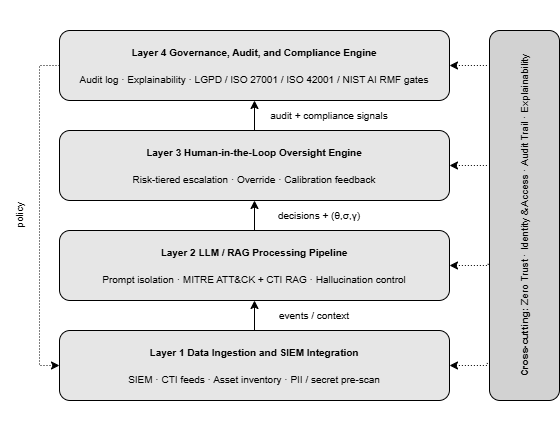
\includegraphics[width=\columnwidth,page=1]{F_concept-1.png}
\caption{SHIELD-AI six-layer governance architecture.
  Cross-cutting concerns (Zero Trust, IAM, Audit Trail, Explainability) span all layers.
  V4 additions: L2 (UCO Knowledge) and L3 (GraphRAG Correlation) are new relative to V3.}
\label{fig:f1arch}
\end{figure}

\subsection{GraphRAG Correlation Engine}
\label{ssec:graphrag}

\subsubsection{Motivation}
Conventional RAG retrieves documents by vector proximity. SOC threat analysis imposes
requirements that vector similarity cannot satisfy: (1) \emph{multi-hop relational reasoning}
(determining T1059$\to$T1078$\to$T1003 requires graph traversal, not similarity lookup);
(2) \emph{contextual entity linkage} (``PowerShell on DC01'' requires knowing DC01 is the AD
domain controller, with an anomalous authentication 6 min earlier -- context in the Asset
Graph, not any document); (3) \emph{explainable inference chains} (audit-readiness requires
explicit paths, not ``the LLM retrieved similar documents'').

\subsubsection{Formal Specification}

\begin{definition}[Knowledge Graph $\mathcal{G}$]
\label{def:kg}
The SHIELD-AI Knowledge Graph is a typed, directed multigraph
$\mathcal{G} = (V, E, \tau_V, \tau_E)$ where $V$ is a set of UCO-typed entity nodes
(types: \textsc{Host}, \textsc{User}, \textsc{IP}, \textsc{Domain}, \textsc{Technique},
\textsc{Tactic}, \textsc{IOC}, \textsc{Campaign}, \textsc{Asset}, \textsc{Incident});
$E \subseteq V \times V$ is a set of typed directed edges;
$\tau_V: V \to \mathcal{T}_V$ assigns a UCO type to each node; and
$\tau_E: E \to \mathcal{T}_E$ assigns a relation type to each edge
(\textsc{UsedBy}, \textsc{ConnectedTo}, \textsc{Implements},
\textsc{AssociatedWith}, \textsc{Escalates}).
\end{definition}

\begin{definition}[GraphRAG Path Confidence $\rho$]
\label{def:graphrag}
Let $q$ be an analytical query and $\Pi = \langle v_0, e_1, v_1, \dots, e_n, v_n \rangle$
a path in $\mathcal{G}$ retrieved by the Correlation Engine. The GraphRAG path confidence is:
\begin{equation}
\rho(\Pi, q) = \prod_{i=1}^{n} w(e_i) \cdot \cos(\mathbf{q}, \mathbf{v}_n),
\label{eq:rho}
\end{equation}
where $w(e_i) \in [0,1]$ is the edge weight (source trust, temporal recency, IOC confidence),
and $\cos(\mathbf{q}, \mathbf{v}_n)$ is the cosine similarity between query and terminal
node embeddings. The overall confidence is
$\rho = \max_{\Pi \in \mathcal{P}(q)} \rho(\Pi, q)$.
\end{definition}

\subsubsection{Concrete SOC Example: Multi-hop Alert Correlation}
Consider the alert: \emph{``PowerShell.exe executed on server DC01''}.

\noindent\textbf{With conventional RAG (L4 only):} Retrieves documents about PowerShell.
LLM produces a generic T1059 response with no host-specific context. Audit trail: ``LLM
retrieved 5 documents mentioning PowerShell.''

\noindent\textbf{With GraphRAG (L2--L3):} The Correlation Engine traverses $\mathcal{G}$
in $\leq 3$ hops:
\begin{align*}
&\texttt{User:alice} \xrightarrow{\textsc{AuthTo}} \texttt{Host:DC01} \xrightarrow{\textsc{Ran}}
\texttt{Proc:pwsh} \\
&\quad\xrightarrow{\textsc{MatchesIOC}} \texttt{IOC:APT29}
\xrightarrow{\textsc{Implements}} \texttt{T1059} \\
&\quad\xrightarrow{\textsc{ChainedWith}} \texttt{T1078}
\xrightarrow{\textsc{ChainedWith}} \texttt{T1003}
\end{align*}
Additional context: alice authenticated anomalously to DC01 6 min before the alert; DC01
is typed \textsc{DomainController} in the Asset Graph; the IOC cluster is associated with
campaign APT29:CozyBear-2025. L6 audit record contains the explicit path $\Pi$ and
$\rho = 0.87$.

\subsection{Calibration Bound and Honest Limits}
Under non-adversarial conditions with positive correlation between the reliability quadruple
and correctness, $P(\neg H \mid R = r) \geq r$. This bound does \emph{not} hold under prompt
injection \cite{liu2024formalizing,zou2023universal}, which inflates apparent reliability
while suppressing correctness. L4 controls (sanitization, instruction--data separation,
output filtering) operate \emph{before} $R$ is computed and aim to restore the bound's
applicability. Residual risk is the principal motivation for HITL as an architectural primitive.

\paragraph{Adversarial-uncertainty mandatory-HITL rule.}
When inter-signal disagreement $\Delta = |\sigma - \gamma| > 0.25$, or
$\gamma - \gamma' > 0.15$, PC3 forces HITL regardless of composite $R$.
Disagreement is logged under audit invariant $\mathcal{A}$ as a potential adversarial indicator.

\subsection{Decision-Theoretic HITL Routing}
\label{ssec:hitl}

Given cost-benefit parameters $b, c_{\text{err}}, c_{\text{analyst}}, \lambda, c_{\text{miss}}$,
the expected utilities are:
\begin{align}
\mathcal{U}_{\text{auto}}(r) &= r \cdot b - (1-r) \cdot c_{\text{err}}, \\
\mathcal{U}_{\text{HITL}}(r) &= b - c_{\text{analyst}} - \lambda, \\
\mathcal{U}_{\text{reject}}(r) &= -c_{\text{miss}}.
\end{align}
Setting $\mathcal{U}_{\text{auto}} = \mathcal{U}_{\text{HITL}}$ yields the optimal threshold:
\begin{equation}
r^*_{\text{auto/HITL}} = \frac{b + c_{\text{err}} - c_{\text{analyst}} - \lambda}{b + c_{\text{err}}}.
\label{eq:threshold}
\end{equation}
Routing thresholds are functions of organizational policy rather than ad-hoc constants,
making them auditable to regulators (Theorem~\ref{thm:routing}).

\begin{algorithm}[!t]
\caption{PC3 -- Human Validation and Hallucination Control}
\label{alg:pc3}
\SetAlgoLined
\DontPrintSemicolon
\KwIn{LLM output \texttt{out}; quadruple $(\theta,\sigma,\gamma,\rho)$;
  policy $\Pi=(\tau_{\text{auto}},\tau_{\text{review}},\mathcal{D}_{\text{deny}},\mathcal{T}_{\text{sens}})$}
\KwOut{route $\in$ \{AUTO, HITL, REJECT\}; audit record $a$}
$R \gets \omega_\theta\theta + \omega_\sigma\sigma + \omega_\gamma\gamma + \omega_\rho\rho$\;
$\Delta \gets |\sigma - \gamma|$\;
\If{\textnormal{out} $\in \mathcal{D}_{\text{deny}}$}{route $\gets$ REJECT}
\ElseIf{\textnormal{out} $\in \mathcal{T}_{\text{sens}}$ \textbf{or} $\Delta > 0.25$}{route $\gets$ HITL}
\ElseIf{$R \geq \tau_{\text{auto}}$ \textbf{and} $\gamma' \geq \tau_{\text{auto}}$}{route $\gets$ AUTO}
\ElseIf{$R \geq \tau_{\text{review}}$}{route $\gets$ HITL}
\Else{route $\gets$ REJECT}
$a \gets \langle$input, prompt, graph\_path, out, $\theta,\sigma,\gamma,\gamma',\rho$, route, analyst, $t\rangle$\;
write $a$ to L6 audit store (append-only, Merkle-chained)\;
\Return (route, $a$)
\end{algorithm}

\subsection{Cross-Standard Control Mapping}
\label{ssec:mapping}

Table~\ref{tab:mapping} aligns SHIELD-AI controls to seven external standards. The mapping
was constructed via a four-step procedure: ontology alignment, double coding by independent
coders, inter-rater reconciliation, and conflict resolution for competing requirements
(e.g., LGPD erasure vs. sectoral retention). Full mapping in the supplementary TSV (OP7).

\begin{table*}[!t]
\renewcommand{\arraystretch}{1.2}
\caption{Cross-standard control mapping (excerpt). Full mapping in supplementary material.}
\label{tab:mapping}
\centering
\scriptsize
\begin{tabular}{lllllllll}
\toprule
\textbf{Control} & \textbf{ATT\&CK} & \textbf{ATLAS} & \textbf{CSF 2.0} & \textbf{OWASP LLM} & \textbf{OWASP A.} & \textbf{27001} & \textbf{42001} & \textbf{LGPD} \\
\midrule
Input sanitization   & n/a    & AML.T0051 & PR.DS-2 & LLM01 & A1  & A.8.27 & 6.1   & Art.46 \\
RAG verification     & n/a    & AML.T0043 & DE.AE-2 & LLM09 & n/a & A.8.16 & 7.4   & Art.6  \\
Self-consistency     & n/a    & AML.T0043 & DE.AE-3 & LLM09 & n/a & A.8.16 & 7.4   & Art.6  \\
GraphRAG path audit  & n/a    & AML.T0043 & DE.AE-2 & LLM09 & A8  & A.5.28 & 8.4   & Art.37 \\
Tool allowlist       & T1059  & AML.T0048 & PR.AC-4 & LLM06 & A2  & A.8.4  & 8.2   & Art.46 \\
Output filtering     & n/a    & AML.T0050 & DE.CM-1 & LLM02 & A6  & A.8.21 & 7.4   & Art.46 \\
Audit log (Merkle)   & n/a    & n/a       & PR.PT-1 & LLM07 & A8  & A.5.28 & 8.4   & Art.37/48 \\
HITL escalation      & n/a    & AML.M0011 & GV.RM-5 & LLM06 & A4  & A.5.4  & 6.1.3 & Art.20 \\
PII pre-scan         & n/a    & n/a       & PR.DS-1 & LLM02 & n/a & A.8.10 & 7.5.3 & Art.46 \\
LGPD compliance gate & n/a    & n/a       & GV.SC-2 & n/a   & n/a & A.5.34 & 6.1.4 & Art.46--48 \\
Identity/Zero-Trust  & T1078  & n/a       & PR.AC-1 & LLM02 & A3  & A.5.15 & 8.2   & Art.46 \\
\bottomrule
\end{tabular}
\end{table*}

\subsection{Properties and Proofs}
\label{ssec:properties}

\begin{lemma}[Audit Completeness]
\label{lem:audit}
Under audit invariant $\mathcal{A}$ and three engineering invariants---%
\textbf{E1} append-only persistence (WORM/immutable schema),
\textbf{E2} cryptographic chaining (Merkle-style with HSM signing),
\textbf{E3} time-monotone clock with bounded skew $\delta$---%
every $d \in \mathcal{D}$ emitted with route $\in \{\text{AUTO},\text{HITL},\text{REJECT}\}$
has an audit record $a$ containing sufficient information to reconstruct $d$, including the
originating input, prompt, graph path, output, reliability quadruple, and routing decision.
\end{lemma}
\begin{proof}
By construction of PC3 (Alg.~\ref{alg:pc3}), every audit record is the tuple
$\langle$input, prompt, graph\_path, output, $\theta,\sigma,\gamma,\gamma',\rho$,
route, analyst, timestamp$\rangle$.
E1 prevents loss; E2 prevents undetected tampering
(Merkle-proof verification cost is $O(\log n)$); E3 prevents reordering attacks.
\end{proof}

\begin{theorem}[Compliance Preservation under Control Composition]
\label{thm:compliance}
Let $c_1, c_2 \in \mathcal{C}$ with LGPD coverage $\geq \alpha$ each. If
$\mathrm{NonInterf}(c_1, c_2)$ (i.e., $\mathrm{Req}(c_1) \subseteq \mathrm{Req}(c_1 \circ c_2)$)
holds, then $\mathrm{LGPD\text{-}coverage}(c_1 \circ c_2) \geq \alpha$.
\end{theorem}
\begin{proof}[Proof sketch]
By the non-interference precondition, $\mathrm{Req}(c_1) \subseteq \mathrm{Req}(c_1 \circ c_2)$.
Let $L \subseteq \mathrm{Req}(c_1)$ be the LGPD Articles 46--48 subset \cite{lgpd2018}.
Then $L \subseteq \mathrm{Req}(c_1 \circ c_2)$, hence coverage is preserved.
Conflicting requirements (LGPD erasure vs. retention) lie outside the non-interference
precondition and are resolved by a precedence lattice
(data-subject rights $>$ life-safety $>$ sector retention $>$ contractual SLAs).
\end{proof}

\begin{theorem}[Policy-Derivable HITL Routing]
\label{thm:routing}
Given cost-benefit parameters $(b, c_{\text{err}}, c_{\text{analyst}}, \lambda, c_{\text{miss}})$
and reliability $R$, the optimal action under expected-utility maximization is determined by the
thresholds in Eq.~\eqref{eq:threshold}: thresholds are functions of organizational policy,
not ad-hoc constants.
\end{theorem}

% =====================================================================
\section{Governance Metrics}
\label{sec:metrics}

We define four metric families: \emph{effectiveness} (DR, FPR, FNR, MTTD, MTTR, AFI),
\emph{AI safety} (Hallucination Rate HR \cite{ji2023hallucination}, Consistency Score CS
\cite{manakul2023selfcheckgpt}, Prompt Injection Resistance PIR, Explainability Score XS),
\emph{compliance} (LGPD-coverage \cite{lgpd2018,anpd15}, ISO-coverage \cite{iso27001,iso42001}),
and \emph{auditability} (Audit Log Completeness ALC, Human Override Rate HOR, Decision
Traceability Score DTS). The \emph{Composite Governance Score} is:
\begin{equation}
\text{CGS} = \sum_{k=1}^{K} w_k \cdot \text{norm}(m_k), \quad \sum_k w_k = 1.
\end{equation}
Default weights (Effectiveness 0.25, AI safety 0.30, Compliance 0.20, Auditability 0.25)
are derived from NIST AI RMF function priorities \cite{nist2023airmf,nist2024genai}; the
derivation procedure is documented in the supplementary material so deployments can re-derive
weights from their own priority structure.

% =====================================================================
\section{Critical-Sector Application Scenarios}
\label{sec:scenarios}

\subsection{Scenario A: Healthcare SOC under LGPD}
Healthcare ransomware risk is documented quantitatively \cite{neprash2022ransomware,
jama2024ransomware,neprash2024changehealthcare}; in Brazil, RNDS digitalization creates
analogous exposure governed by LGPD with elevated sensitivity for health data.

SHIELD-AI instantiation: L1 ingests EHR/RNDS logs through the PII gate; L2 Knowledge Layer
runs GraphRAG over ATT\&CK augmented with health-CTI; L5 escalation thresholds are tuned with
elevated $c_{\text{err}}$ (patient-safety stakes); L6 enforces LGPD Art.~46--48 and ANPD
Resolution 15/2024 incident-notification timing (3 business days, extendable to 20)
\cite{anpd15}.

\subsection{Scenario B: Government and Critical Infrastructure}
Critical infrastructure accounts for 70\% of IBM-investigated incidents \cite{xforce2025};
manufacturing is the most-attacked sector for the fourth consecutive year; destructive cloud
campaigns are up 87\% \cite{mddr2025}. SHIELD-AI instantiation: L6 anchors to NIST CSF 2.0
\cite{nist2024csf} and ISO 27001 \cite{iso27001}; L1 supports SCADA/OT log ingestion; L5
thresholds tune the latency penalty $\lambda$ to OT availability constraints
\cite{nsa2024deploying}.

% =====================================================================
\section{Evaluation}
\label{sec:eval}

\subsection{Scenario Analysis}

\begin{table}[!t]
\renewcommand{\arraystretch}{1.2}
\caption{Scenario evaluation (author-assigned Likert 1--5; protocol pre-registered).}
\label{tab:scenarioscores}
\centering
\scriptsize
\resizebox{\columnwidth}{!}{%
\begin{tabular}{lccccc}
\toprule
& \makecell{Threat\\cov.} & \makecell{LLM\\risk} & \makecell{Reg.\\cov.} & \makecell{HITL\\approp.} & \makecell{Audit\\compl.} \\
\midrule
Scenario A (Healthcare) & 5 & 4 & 5 & 5 & 5 \\
Scenario B (Gov./OT)    & 4 & 4 & 4 & 4 & 5 \\
\bottomrule
\end{tabular}}%
\end{table}

Scenario A scores Threat coverage 5/5 (ransomware/AI-augmented attacks detectable via L1/L2),
LLM-risk 4/5 (vishing upstream of SOC ingestion not addressed), Regulatory 5/5 (LGPD
operationalized at L6), HITL 5/5 (elevated $c_{\text{err}}$ produces conservative thresholds),
Auditability 5/5 (Lemma~\ref{lem:audit}). Scenario B is one point lower on threat coverage
(OT-specific TTPs need an ATT\&CK for ICS extension), regulatory coverage (sector regulators
ANATEL/ANEEL not covered), and HITL (latency parameter $\lambda$ must be tuned).

\subsection{Reproducible Reference Experiment}
\label{ssec:empirical}

\textbf{Setup.} We implemented SHIELD-AI as a Python package and evaluated it on a
\emph{synthetic} labelled flow dataset mirroring the CICIDS-2017 schema (24 CICFlowMeter
features, 14 attack classes plus benign), generated programmatically calibrated against
descriptive statistics from \cite{sharafaldin2018cicids}. We generated $n{=}60{,}000$ flows
(30\% attack ratio, 75/25 train/test split, seed 42). Three L4 configurations run in parallel:
rule-based (Sigma-style pattern match), Random Forest (200 trees, max-depth 18, balanced
subsampling), and the SHIELD-AI LLM/RAG path (RF prior + $k{=}5$ self-consistency samples
at temperature 0.45 + TF-cosine retriever over hand-coded ATT\&CK KB). PC3 was configured
with $r^*_{\text{auto}} = 0.80$ (from $b{=}1$, $c_{\text{err}}{=}2$, $c_{\text{analyst}}{=}0.3$,
$\lambda{=}0.3$). L6 appended each decision to an HMAC-signed log batched into Merkle roots
of size 1024. Experiments ran on a commodity laptop (Apple M-series, 16~GiB RAM, no GPU).

\textbf{Headline results.} Table~\ref{tab:exp-headline} reports the binary attack/benign
performance, routing distribution, and audit invariants. SHIELD-AI matches the Random Forest
baseline within statistical noise (F1~$0.984$ vs.~$0.985$; AUC~$0.998$ vs.~$0.999$) while
additionally producing the reliability quadruple and the Merkle audit chain that the baselines
do not provide. The rule-based detector requires a $\sim$94$\times$ higher FPR at equal F1.
At aggregate level SHIELD-AI auto-resolves 69.0\% of decisions, escalates 29.7\% to analysts,
and safely rejects 1.3\%.

\begin{table}[!t]
\renewcommand{\arraystretch}{1.2}
\caption{Reference-experiment headline results on $15{,}000$ synthetic test flows (seed 42).
Routing refers to PC3 (AUTO/HITL/REJECT). Audit: chain verified for all $15{,}000$ records
(15 Merkle roots); 50/50 spot-check PASS.}
\label{tab:exp-headline}
\centering
\scriptsize
\begin{tabular}{lccccl}
\toprule
\textbf{System} & \textbf{F1} & \textbf{FPR} & \textbf{AUC} & \textbf{Macro-F1} & \textbf{Routing} \\
\midrule
Rule-based       & 0.516 & 0.375 & 0.750 & 0.121 & n/a \\
Random Forest    & 0.985 & 0.004 & 0.999 & 0.513 & n/a \\
SHIELD-AI (full) & 0.984 & 0.004 & 0.998 & 0.497 & 69/30/1\% \\
\bottomrule
\end{tabular}
\end{table}

\textbf{Key observations.} (1) The adversarial-aware groundedness $\gamma'$ (mean 0.575,
$p_{50}$=0.570, $p_{10}$=0.255, $p_{90}$=0.766) is the principal differentiator in PC3
routing: classes with clean ATT\&CK lexical alignment (DDoS$\to$T1498) reach
$\gamma' \in [0.70, 0.85]$; PortScan ($\to$T1046 ``Network Service Discovery'') receives
lower $\gamma'$ and is routed predominantly to HITL -- the intended behavior for
ambiguous labels. (2) L6 audit latency averages 0.014~ms/record, well within a 50~ms budget.
(3) Chain re-derivation passes for all 15{,}000 records; tamper tests (unit test
\texttt{test\_audit\_chain.py}) detect a single bit-flip in any record's predicted label.

\textbf{Scope and limitations.} This is a reproducible reference experiment, not a field
trial: the LLM is simulated by perturbed RF priors; the synthetic generator preserves
CICIDS-2017 schema but not adversarial co-evolution; absolute threshold values must be
re-calibrated against a production LLM before deployment. Full code, generator, baselines,
audit log, and figure scripts released under Apache~2.0 at the companion repository
(DOI to be added on camera-ready per OP7).

\subsection{Threats to Validity}
Following \cite{wohlin2012experimentation}: \emph{Construct} -- framework concepts may not
capture all SOC governance dimensions (mitigated by multi-source grounding). \emph{Internal}
-- scenario design may favor the framework (mitigated by scenarios drawn from independent
threat intel). \emph{External} -- two scenarios limit generalizability (mitigated by spanning
healthcare and government; further sectors as future work). \emph{Conclusion} -- ENISA
comparison is qualitative (explicit criteria matrix with declared limitations).

% =====================================================================
\section{Discussion}
\label{sec:discussion}

\subsection{Implications for Practitioners}
Principal finding: integrated governance is feasible and aligns with multi-standard compliance
simultaneously. Practitioners should prioritize L6 (audit, compliance) and L5 (HITL) before
scaling L4 (LLM/RAG) autonomy -- a sequencing that inverts the ``add AI first, govern later''
pattern documented for 63\% of organizations \cite{ibm2025costbreach}.

\subsection{Acknowledged Limitations}
Seven limitations are explicitly acknowledged:
(A1) The contribution is an integration, not a creation of new risks or controls.
(A2) HITL cost parameters $(b, c_{\text{err}}, \ldots)$ are policy choices with order-of-magnitude
uncertainty; Theorem~\ref{thm:routing} guarantees policy-derivable routing, not optimal routing.
(A3) L6 staffing assumes mid-to-large SOCs; a ``L6-light'' variant for small SOCs is future work.
(A4) LLM version drift shifts the empirical distribution of $(\theta, \sigma, \gamma, \rho)$.
(A5) Single-agent semantics; multi-agent cascading \cite{owasp2025agentic} requires extension.
(A6) Vishing is upstream of SOC ingestion and outside L1's scope.
(A7) \emph{Compliance theater}: adoption without operationalized KPIs is an explicit risk.

\subsection{Research Agenda}
Nine open problems:
(OP1) Quantitative validation via historical-incident replay in live SOCs.
(OP2) LLM-on-LLM adversarial dynamics \cite{owasp2025agentic,lga2026}.
(OP3) Cross-jurisdictional mapping (LGPD/GDPR/CCPA/DPDP).
(OP4) Continuous-learning HITL without drift.
(OP5) Cost-effectiveness (TCO vs. analyst hours).
(OP6) Standards co-evolution response protocol.
(OP7) Open-source reference release (current companion repo, camera-ready DOI).
(OP8) Empirical calibration of reliability weights $(\omega_\theta, \omega_\sigma, \omega_\gamma,
\omega_\rho)$ and $\gamma$ sub-signal weights across LLM families.
(OP9) Field pilots, KPI programmes (Compliance Theater Index), and adversarial purple-team
evaluation \cite{liu2024formalizing,zou2023universal}.

% =====================================================================
\section{Conclusion}
\label{sec:conclusion}

SHIELD-AI integrates a dual-use GenAI taxonomy, a probabilistic risk model with reliability
quadruple $\langle\theta,\sigma,\gamma,\rho\rangle$, a six-layer reference architecture with
HITL as architectural primitive and a GraphRAG Correlation Engine grounded in UCO, and a
cross-standard control mapping across seven standards including LGPD. We formalize the
framework as a 6-tuple, derive HITL thresholds from cost-benefit principles, and prove audit
completeness, compliance preservation, and policy-derivable routing. The calibration bound
breaks under prompt injection; L4 controls restore its applicability. Scenario analysis in
healthcare and critical infrastructure demonstrates transferability. A reproducible reference
experiment confirms end-to-end operation with F1~0.984, AUC~0.998, and verified Merkle audit
chain. Future work includes operational empirical evaluation, multi-agent semantics, and
cross-jurisdictional compliance extension.

% =====================================================================
\section*{Acknowledgment}
The authors acknowledge the Amazon Foundation for Research Support (FAPESPA), the
Information and Communication Technology Company of the State of Pará (PRODEPA), the
Government of the State of Pará, and the Federal Government of Brazil for their
institutional and financial support, which were essential to enabling the infrastructure,
experimental testbeds, and interinstitutional collaborations underpinning this research.
Special thanks are extended to the spinoff SEC365 and to the Laboratory of
Informatics and Computing of the Amazon (LICA/UFRA), whose teams played a decisive role
in the development, validation, and technical implementation of this work.
The authors also acknowledge the High-Performance Computing and Artificial Intelligence
Center (CCAD-IA/UFPA) and the National Education and Research Network (RNP) for
providing computing resources and technical assistance during the experimental phases.
This work was further supported by the National Institute of Science and Technology in
Artificial Intelligence Applied to Smart and Sustainable Cities in the Brazilian Amazon
(INCT iAmazonia).

% =====================================================================
\section*{Declaration of Generative AI Use}
The authors used large language model (LLM) assistance in the preparation of this
manuscript, including support for manuscript drafting and structural refinement,
Python code scaffolding for the SHIELD-AI pipeline
(\texttt{layer1\_ingest.py}, \texttt{layer2\_llm\_rag.py}, \texttt{layer3\_hitl.py},
\texttt{layer4\_audit.py}) and the end-to-end experiment runner
(\texttt{run\_experiment.py}), \LaTeX{} formatting, and bibliography organisation.
This use is disclosed in accordance with IEEE's Authorship and AI Policy.
All scientific contributions --- including the SHIELD-AI framework design, the
six-layer reference architecture, formal definitions and proofs, the PC3 routing
algorithm, experimental methodology, data analysis, and conclusions --- are the sole
responsibility of the human authors.
The reference experiment (Section~\ref{sec:eval}) was executed by automated scripts
without LLM involvement in data collection or scoring.
Benchmark data are derived from the publicly available CICIDS-2017 dataset and
synthetic extensions generated and validated by the authors; no benchmark figures
were produced or altered by the LLM assistant.
The replication package (code, results, and figures) is available at
\url{https://github.com/ufxa/SHIELD-AI-A-Multi-Layer-Governance-Framework}.

% =====================================================================
\bibliographystyle{IEEEtran}
\bibliography{references}

\end{document}
